\chapter{界面设计}
\section{客户端界面}
之前已经多次提到过,普通用户和开发者共用一个客户端。

界面示例见图\ref{fig:ui_desktop_home}、\ref{fig:ui_desktop_app}、\ref{fig:ui_mobile_home}、\ref{fig:ui_mobile_app}。

\begin{figure}[ht]
	\centering
	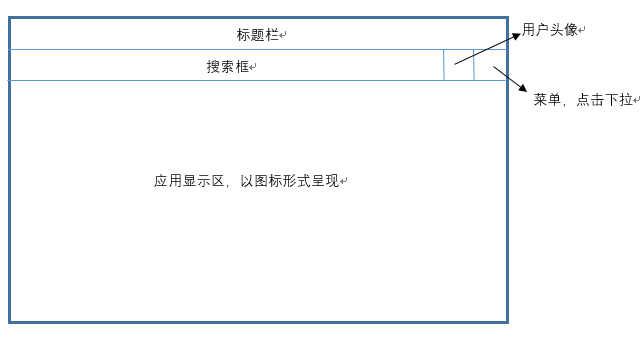
\includegraphics[width=10cm]{ui_desktop.png}
	\caption{桌面端应用商店主界面} \label{fig:ui_desktop_home}
\end{figure}

\begin{figure}[ht]
	\centering
	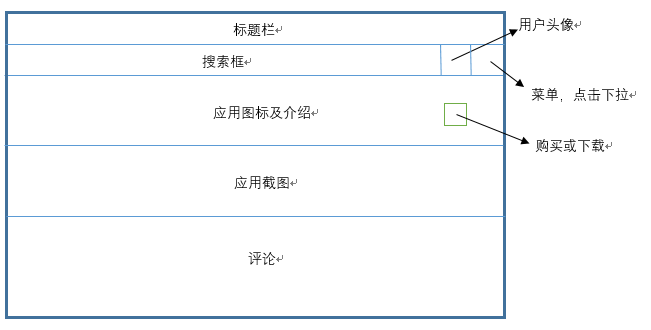
\includegraphics[width=10cm]{ui_desktop1.png}
	\caption{桌面端应用商店应用界面} \label{fig:ui_desktop_app}
\end{figure}

\begin{figure}[ht]
	\centering
	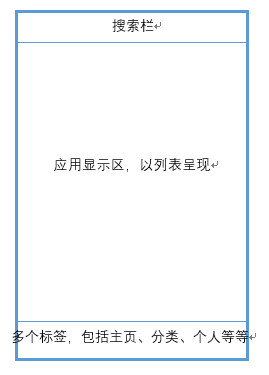
\includegraphics[width=6cm]{ui_mobile.png}
	\caption{移动端应用商店主界面} \label{fig:ui_mobile_home}
\end{figure}

\begin{figure}[ht]
	\centering
	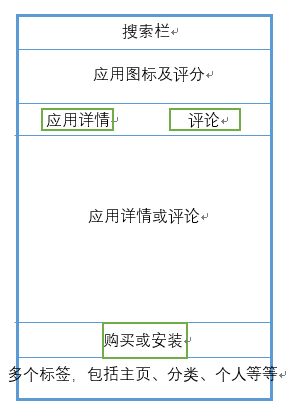
\includegraphics[width=6cm]{ui_mobile1.png}
	\caption{移动端应用商店应用界面} \label{fig:ui_mobile_app}
\end{figure}

以上只列出了部分用户界面。最终的用户界面可能与目前的示例有所偏差。

\section{服务器端界面}
服务器端不需要界面。管理员直接使用命令行交互。

